\documentclass{beamer}
% \documentclass[handout]{beamer}


\setbeameroption{show notes on second screen=right}
% \setbeameroption{show only notes}
\setbeamercolor{frame number in head/foot}{fg=black}
\setbeamerfont{frame number in head/foot}{size=\small}
% \setbeamertemplate{note page}[plain]
\setbeamertemplate{navigation symbols}{}
\setbeamertemplate{footline}[frame number]


% \setbeamercolor{frametitle}{fg=white}
% \setbeamercolor{background canvas}{bg=black}
% \setbeamercolor{normal text}{fg=white}

\usepackage{hyperref,xcolor,tikz,listings}
\usepackage{amsmath,amssymb,amsfonts,amsthm}
\usepackage{multirow,longtable,booktabs,array}
% fonts
\usepackage{fontspec}
\usepackage[T1]{fontenc}
\usepackage[tt=false, type1=true]{libertine}
\usepackage[libertine]{newtxmath}
% misc
\usepackage{xfrac}
\usepackage{graphicx}
\usepackage{float,caption,subcaption} % support \subfigure and \begin{figure}[H] https://tex.stackexchange.com/a/299246 


\usepackage{import}
\usepackage{changepage}
\usepackage{mathtools} % \xmapsto

\definecolor{red}{HTML}{C63A44}
\usetikzlibrary{decorations.pathreplacing}
\captionsetup{justification=raggedright,singlelinecheck=false}
\hypersetup{colorlinks=true,linkcolor=blue,urlcolor=cyan}

\newcommand\sube\subseteq
\newcommand\supe\supseteq
\renewcommand\sup\supset
\newcommand\gt>
\newcommand\lt<
\renewcommand\ge\geqslant 
\renewcommand\geq\geqslant 
\renewcommand\le\leqslant 
\renewcommand\leq\leqslant 
\newcommand\rarr\rightarrow

\setmonofont{iosevka-custom-regular.ttf}
\setlength\parindent{0pt}

\graphicspath{{figures/}}
\newcommand\g[2][0.2]{\raisebox{-0.45\height}{\includegraphics[width=#1\columnwidth]{#2}}}
\newcommand\n[2][1]{\note<.#1>[item]{#2}}

\title{A Computational Approach to String Figures}
\date{2023-11-29}
\author{Yulong Liu}
\begin{document}
\maketitle


\section{String Figures}

\begin{frame}{\secname}
\begin{itemize}
    \item Designs formed from a loop of string
    \item Commonly known as a children's game
\end{itemize}

\pause People have been playing with the string around the world for millennia.

\begin{itemize}[<+(1)->]
    \item  Entertainment during polar nights in the Arctic region
    \item  Storytelling and illustrating scenes from myths and legends
\end{itemize}

\textcolor{red}{todo insert 3 images of strings figures from the encyclopedia: the star, something i can do, something i cant do}
\end{frame}

\note[itemize]{
\item the native inhabitants in the arctic region play string figures for entertainment durong polar nights
\item the indigenous people in New Zealand play string figures for storytelling and illustrating scenes from myths and legends
\item and i play string figures when overleaf takes forever to compile my slides
}


\begin{frame}{A Computational Approach}
String figures take a lot of steps to make

\begin{itemize}[<+(1)->]
    \item  Start with an initial position
    \item  Apply a sequence of moves
    \item  Each move transforms a string figure to another
\end{itemize}

\pause String figures computations

\begin{itemize}[<+(1)->]
    \item  Represent string figures: simple, precise
    \item  Apply moves directly to the representations
\end{itemize}

\pause Motivation

\begin{itemize}[<+(1)->]
    \item Do string figures on paper
    \item Computer simulations \& animations
\end{itemize}

\end{frame}

\note[itemize]{
\item (take steps) for example, to make the star, we start with this initial position, and then apply two simple moves of picking a segment of the string 
\item (mot) clear way of describing how to make string figures
\item (mot) teach computers how to play string figures
\item (record) store in computer, as database
\item simliar to music scores, rubiks cubes
\item one effective way of describing string figures is to draw them, as string diagrams
}
\newcommand\w[1]{\includegraphics[width=0.3\textwidth]{#1}}
\section{Representation}

\subsection{Diagrams}
\begin{frame}{\secname: \subsecname}

Fingers are named $L1,\cdots, L5$ and $R1,\cdots,R5$ from thumb to pinky

\begin{itemize}
    \item Ordered from nearest to furthest
 \begin{center}
    $L1\lt L2\lt L3\lt L4\lt L5$\\
    $R1\lt R2\lt R3\lt R4\lt R5$    
    \end{center}
\end{itemize}

String segments are named by finger $F\in\{L1,\cdots, L5,R1,\cdots,R5\}$
\begin{itemize}
    \item $Fn$ is the near string, $Ff$ is the far string
    \item $Lp$ and $Rp$ are palmar strings
\end{itemize}
\end{frame}

\begin{frame}{\secname: \subsecname}
\includegraphics[width=0.9\columnwidth]{figures/open.png}
% \begin{figure}\centering
% \def\svgwidth{0.9\columnwidth}
% \input{figures/open.pdf_tex}
% \end{figure}
\end{frame}

\subsection{Linear Sequences}
\begin{frame}{\secname: \subsecname}
Two components
\begin{itemize}
    \item Fingers that hold the string
    \item Crossings between two segments
\end{itemize}

Diagram $\to$ linear sequence

\begin{itemize}
    \item Start with left nearest finger and travel clockwise
    \item Visit fingers and crossings
\end{itemize}

\end{frame}

\begin{frame}{\secname: \subsecname}
\begin{center}
    \includegraphics[width=0.7\columnwidth]{figures/open.png}
\end{center}
$$L1:L5:R2$$
\end{frame}

\begin{frame}[t]{Linear Sequences with Crossings}
Diagram $\to$ linear sequence
\begin{itemize}
    \item Name each crossing as $x_i$ for some $i$
    \item Visit overcrossing $\implies$ write $x_i(o)$
    \item Visit undercrossing $\implies$ write $x_i(u)$
\end{itemize}

\end{frame}

\begin{frame}{Linear Sequences with Crossings}
\begin{adjustwidth}{-1.5em}{-1.5em}
\begin{center}
\includegraphics[width=0.7\columnwidth]{figures/star-pick.png}
\end{center}

$$
L1:x_2(o):R5:x_1(o):L5:x_1(u):x_2(u):R2
$$
\end{adjustwidth}
\end{frame}

\subsection{Identifying String Segments }

\begin{frame}{\subsecname from Linear Sequences}
\begin{adjustwidth}{-1.5em}{-1.5em}
Consider a left-hand finger $L_i$ in the sequence

\begin{itemize}
    \item Traverse clockwise \raisebox{-0.45\height}{\includegraphics[width=0.2\textwidth]{figures/leftcw.png}} $\implies \ldots:[n] L_i [f]:\ldots$
    \item Traverse counterclockwise \raisebox{-0.45\height}{\includegraphics[width=0.2\textwidth]{figures/leftccw.png}} $\implies\ldots: [f] L_i [n]:\ldots$
\end{itemize}

Similarly for finger $R_i$ on the right hand

\begin{itemize}
    \item \raisebox{-0.45\height}{\includegraphics[width=0.2\textwidth]{figures/rightcw.png}} $\implies \ldots:[f]R_i[n]:\ldots$
    \item\raisebox{-0.45\height}{\includegraphics[width=0.2\textwidth]{figures/rightccw.png}} $\implies\ldots:[n]R_i[f]:\ldots$
\end{itemize}
\end{adjustwidth}
\end{frame}

\begin{frame}{\subsecname: Opposite Hand}
\begin{adjustwidth}{-1.5em}{-1.5em}
Consider $\ldots:L_i:\ldots:R_j:\ldots$
\begin{itemize}
    \item Even number of crossings between $L_i$ and $R_j\implies$ orientation persists\\
    \begin{center}
    \includegraphics[width=0.5\columnwidth]{figures/diff-even.png}
    $$
    [n]L_i[f]:[f]R_j[n]
    $$
    \end{center}
    \item Odd number of crossings between $L_i$ and $R_j\implies$ orientation reverses\\
    \begin{center}
    \includegraphics[width=0.5\columnwidth]{figures/diff-odd.png}
    $$
    [n]L_i[f]:x_1(u):[n]R_j[f]:x_1(o)
    $$
    \end{center}
\end{itemize}
\end{adjustwidth}
\end{frame}

\begin{frame}{\subsecname: Same Hand}
\begin{adjustwidth}{-1.5em}{-1.5em}
Consider $\ldots:L_i:\ldots:L_j:\ldots$

\vfill
\begin{minipage}{0.45\textwidth}
\begin{center}
Even $\implies$ orientation persists\\
\includegraphics[width=0.3\linewidth]{figures/same-even.png}
\end{center}
$$
\scriptstyle
\ldots:[n]L_i[f]:[n]L_j[f]:\ldots
$$
\end{minipage}
\hfill
\begin{minipage}{0.45\textwidth}
\begin{center}
Odd $\implies$ orientation reverses\\
\includegraphics[width=0.3\linewidth]{figures/same-odd.png}
\end{center}
$$
\scriptstyle
\ldots:[n]L_i[f]:x_1(u):[f]L_j[n]:x_1(o):\ldots
$$
\end{minipage}
\end{adjustwidth}
\end{frame}

\begin{frame}[t]{\subsecname: Example}

$$
{L1}:x_2(o):R5:x_1(o):L5:x_1(u):x_2(u):R2
$$

{By convention, the first finger in the linear sequence is clockwise}

\begin{adjustwidth}{-2em}{-2em}
$$
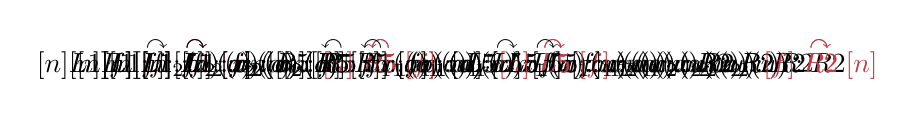
\begin{tikzpicture}
    \node<+> at(0,0){$\stackrel{\phantom\curvearrowright}{L1}:x_2(o):R5:x_1(o):L5:x_1(u):x_2(u):R2$};
    \node<+> at(0,0){${\color{red}\stackrel\curvearrowright{L1}}:x_2(o):R5:x_1(o):L5:x_1(u):x_2(u):R2$};
    \node<+> at(0,0){${\color{red}[n]\stackrel\curvearrowright{L1}[f]}:x_2(o):R5:x_1(o):L5:x_1(u):x_2(u):R2$};
    \node<+> at(0,0){$[n]\stackrel\curvearrowright{L1}[f]:x_2(o):{\color{red}\stackrel\curvearrowleft{R5}}:x_1(o):L5:x_1(u):x_2(u):R2$};
    \node<+> at(0,0){$[n]\stackrel\curvearrowright{L1}[f]:x_2(o):{\color{red}[n]\stackrel\curvearrowleft{R5}[f]}:x_1(o):L5:x_1(u):x_2(u):R2$};
    \node<+> at(0,0){$[n]L1[f]:x_2(o):[n]\stackrel\curvearrowleft{R5}[f]:x_1(o):{\color{red}\stackrel\curvearrowright{L5}}:x_1(u):x_2(u):R2$};
    \node<+> at(0,0){$[n]L1[f]:x_2(o):[n]\stackrel\curvearrowleft{R5}[f]:x_1(o):{\color{red}[n]\stackrel\curvearrowright{L5}[f]}:x_1(u):x_2(u):R2$};
    \node<+> at(0,0){$[n]L1[f]:x_2(o):[n]R5[f]:x_1(o):[n]\stackrel\curvearrowright{L5}[f]:x_1(u):x_2(u):{\color{red}\stackrel\curvearrowright{R2}}$};
    \node<+> at(0,0){$[n]L1[f]:x_2(o):[n]R5[f]:x_1(o):[n]\stackrel\curvearrowright{L5}[f]:x_1(u):x_2(u):{\color{red}[f]\stackrel\curvearrowright{R2}[n]}$};
\end{tikzpicture}
$$
\end{adjustwidth}

$$
\begin{tikzpicture}
    \node<3>at(0,0){\w{figures/leftcw.png}};
    \node<5>at(0,0){\w{figures/rightccw.png}};
    \node<7>at(0,0){\w{figures/leftcw.png}};
    \node<9>at(0,0){\w{figures/rightcw.png}};
\end{tikzpicture}$$
\end{frame}

\begin{frame}{\subsecname: Example}
$$
[n]L1[f]:x_2(o):[n]R5[f]:x_1(o):[n]{L5}[f]:x_1(u):x_2(u):{[f]{R2}[n]}
$$

\begin{center}
\includegraphics[width=0.7\columnwidth]{figures/star-pick.png}
\end{center}
\end{frame}

% \section{Moves}
% \subsection{Twist}
% 
\begin{frame}{\secname: \subsecname}
\pause Two variations: twist towards and twist away
\begin{itemize}[<+(1)->]
    \item Twist the loop on finger $F$ \emph{towards} player: $<F$
    \note<.(1)>[item]{this is the notation}
    \item Twist the loop on finger $F$ \emph{away} from player: $>F$
\end{itemize}
\pause Consider $\ldots:[n]F[f]:\ldots$
\begin{itemize}[<+(1)->]
    \item\g[0.15]{figures/twist-before} $\quad\stackrel{<F}\mapsto\quad$ \g[0.15]{figures/twist-towards}
    $$
    \ldots:[n]F[f]:\ldots\quad\stackrel{<F}\mapsto\quad\ldots:x_1(u):F:x_1(o):\ldots
    $$
    \item \g[0.15]{figures/twist-before} $\quad\stackrel{>F}\mapsto\quad$ \g[0.15]{figures/twist-away}
    $$
    \ldots:[n]F[f]:\ldots\quad\stackrel{>F}\mapsto\quad\ldots:x_1(o):F:x_1(u):\ldots
    $$
    \item $\ldots:[f]F[n]:\ldots\stackrel{<F}\mapsto \ldots:x(o):F:x(u):\ldots$
\note<.(1)->[item]{if we have the far segment coming before the finger, that means we are traversing in the opposite orientation}
    \item $\ldots:[f]F[n]:\ldots\stackrel{>F}\mapsto \ldots:x(u):F:x(o):\ldots$
\end{itemize}

% Storer p382
\end{frame}
\note[itemize]{
\item the transformation of the linear sequence works on right hand too
\item draw right hand ccw $<F$
\item ARE WE OK WITH THIS
\item now we can start describing the most used moves in string figures, pick
}

% \subsection{Pick}
% \begin{frame}{\secname: \subsecname}

Finger $F$ picks a string segment $s$ 

\begin{itemize}
    \item Written as $F(s)$
\end{itemize}

 Four variations:
\begin{itemize}
    \item $F$ passes \emph{over/under} all intermediate segments
    \item $F$ picks $s$ from \emph{above/below}
    \note<.(1)>[item]{(CAMERA) show all 4 cases on $L1:R1$ with $R5(R1n)$}
\end{itemize}

 Examples
\begin{itemize}
    \item "$R5$ passes \emph{over} all intermediate segments and picks $Lp$ from \emph{above}" is denoted  as $\overset\Longleftarrow{R5}(\overline{Lp})$
    \item "$R1$ passes \emph{over} all intermediate segments and picks $R5n$ from \emph{below}" is denoted as $\overrightarrow{R1}(\underline{R5n})$
    \note<.(1)>[item]{the first 2 moves makes the star}
    \item "$R4$ passes \emph{below} all intermediate segments and picks $L1n$ from \emph{below}" is denoted as $\underset\Longleftarrow{R4}(\underline{L1n})$
\end{itemize}
\end{frame}

\note[itemize]{
\item have an arrow above the finger means pass \emph{over}, underarrow means pass \emph{under}
\item an underlined segment means pick the segment from below, overline means from above
\item this notations come from a monograph written by a mathematician Tom Storer
\item Storer says that the single arrow is for same hand pick, and right arrow means finger moves away
\item says that double arrow for opposite hand pick, left arrow means right finger picks left segments
\item the direction of the arrows can be determined by the finger and segment, so its redundant, but i'm following Storer's convention
}

\begin{frame}{\subsecname: Examples}
\note<1>[item]{now lets look at how these different pick moves change the linear sequence}
\begin{adjustwidth}{-2em}{-2em}
Starting with \g{figures/pick-before}$\enspace [n]L1[f]:[f]R1[n]$\\
\begin{minipage}{0.55\columnwidth}
 $\underleftarrow{R5}(\underline{R1n})$ gives \g[0.3]{figures/pick-under-below}\\
$L1:x_1(o):x_2(o):R1:x_2(u):R5:x_1(u)$\\
\vfill
 $\underleftarrow{R5}(\overline{R1n})$ gives \g[0.3]{figures/pick-under-above}\\
$L1:x_1(o):x_2(o):R1:x_2(u):x_3(u):R5:x_3(o):x_1(u)$\\
\end{minipage}
\hfill
\begin{minipage}{0.55\columnwidth}
 $\overleftarrow{R5}(\underline{R1n})$ gives \g[0.3]{figures/pick-over-below}\\
$L1:x_1(u):x_2(u):R1:x_2(o):R5:x_1(o)$\\
\vfill
 $\overleftarrow{R5}(\overline{R1n})$ gives \g[0.3]{figures/pick-over-above}\\
$L1:x_1(u):x_2(u):R1:x_2(o):x_3(u):R5:x_3(o):x_1(o)$\\
\end{minipage}\\
 Observations
\begin{itemize}
    \item A pair of crossings for each intermediate string
    \item $\overleftarrow F(s)$ and $\underleftarrow F(s)$ differ by crossing parity
    \item $F(\overline s)$ and $F(\underline s)$ differ by a twist
\end{itemize}
\end{adjustwidth}
\end{frame}

\note[itemize]{
\item in this case, we always insert the new finger $R5$, at where $R1n$ is in the sequence
\item and insert $x_1$ at $L1f$ and $x_2$ at $R1f$ since intermediate
\item when $F$ moves away, the new twist is away, e.g. $L5:R5$ and pick with $R1$
}


\begin{frame}{\subsecname: Construction}
General steps for applying $F(s)$ to a string figure
\begin{itemize}
    \item Identify intermediate segments
    \item Insert a pair of crossings for each intermediate segment
    \item Insert $F$ at $s$ with crossings
    \item Add twist if pick from above
\end{itemize}

% write operation
\g[0.27]{figures/star-before}
{$\mapsto$\g[0.27]{figures/star-pick}}
{$\mapsto$\g[0.27]{figures/star-pick-twist}}

\note[item]{in this case, suppose i want to apply (WRITE) $\overset\Longleftarrow{R5}(\overline{Lp})$}
\end{frame}
\note[itemize]{
\item this is a visual of what we should expect when we apply the computation, 
\item now we will this without diagrams, working on linear sequences only
}

% \newcommand\name{\subsecname: Construction Example}
\begin{frame}{\name}
$L1:L5:R2\enspace\xmapsto{\overset\Longleftarrow{R5}(\overline{Lp})}\enspace???$

\begin{itemize}
    \item Identify $Lp$\\
    $$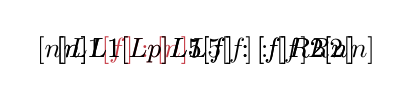
\begin{tikzpicture}
        \node<+> at(0,0){$[n]L1{\color{red}[f]:[n]}L5[f]:[f]R2[n]$};
        \node<+> at(0,0){$[n]L1{\color{red}[Lp]}L5[f]:[f]R2[n]$};
        \node<+-> at(0,0){$[n]L1[Lp]L5[f]:[f]R2[n]$};
    \end{tikzpicture}$$
    \item<+-> Only the segment between $L5$ and $R2$ is intermediate
    $$
      \underline{R2n=L1n}<L1<{\color{red}Lp}=L5n<\underline{L5f=R2f}<{\color{red}R5}
      $$
    
\end{itemize}
\end{frame}

\begin{frame}{\name}
$L1:L5:R2\enspace\xmapsto{\overset\Longleftarrow{R5}(\overline{Lp})}\enspace???$\\
\vfill
Found $L5f=R2f$ as an intermediate segment
\begin{itemize}
    \item<1-> Insert crossings $x_1$ and $x_2$ at intermediate segment
    \note<3>[item]{under because our finger is going above}
    $$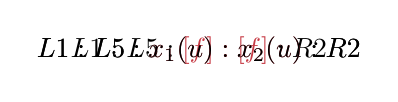
\begin{tikzpicture}
        \node<2> at(0,0){$L1:L5:{\color{red}[f]:[f]}:R2$};
        \node<3> at(0,0){$L1:L5:{\color{red}x_1(u):x_2(u)}:R2$};
        \node<4-> at(0,0){$L1:L5:x_1(u):x_2(u):R2$};
    \end{tikzpicture}$$
    \item<4-> Insert $R5$ at $Lp$ with $x_1$ and $x_2$
    $$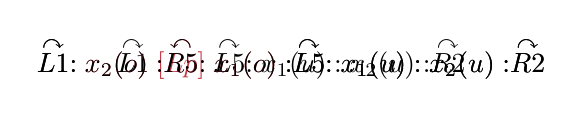
\begin{tikzpicture}
        \node<5> at(0,0){$\stackrel\curvearrowright{L1}{\color{red}[Lp]}\stackrel\curvearrowright{L5}:x_1(u):x_2(u):\stackrel\curvearrowright{R2}$};
        \node<6> at(0,0){$\stackrel\curvearrowright{L1}:{\color{red}x_2(o):\stackrel\curvearrowleft{R5}:x_1(o)}:\stackrel\curvearrowright{L5}:x_1(u):x_2(u):\stackrel\curvearrowright{R2}$};
        \node<7-> at(0,0){$\stackrel\curvearrowright{L1}:x_2(o):\stackrel\curvearrowleft{R5}:x_1(o):\stackrel\curvearrowright{L5}:x_1(u):x_2(u):\stackrel\curvearrowright{R2}$};
    \end{tikzpicture}$$
    $$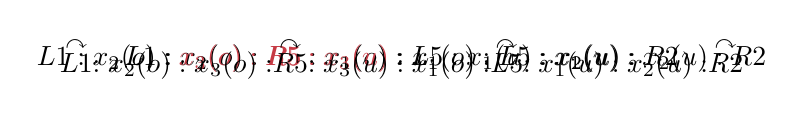
\begin{tikzpicture}
        \node<8> at(0,0){$L1:x_2(o):{\color{red}R5}:x_1(o):L5:x_1(u):x_2(u):R2$};
        \node<9> at(0,0){$L1:x_2(o):{\color{red}x_3(o):R5:x_3(u)}:x_1(o):L5:x_1(u):x_2(u):R2$};
        \node<10-> at(0,0){$\stackrel\curvearrowright{L1}:x_2(o):{x_3(o):\stackrel\curvearrowright{R5}:x_3(u)}:x_1(o):\stackrel\curvearrowright{L5}:x_1(u):x_2(u):\stackrel\curvearrowright{R2}$};
    \end{tikzpicture}$$
\end{itemize}
\end{frame}
\note[itemize]{
\item and this is our final result, lets check with the diagram
}

\begin{frame}{\name}
$$\scriptstyle
L1:L5:R2\enspace\xmapsto{\overset\Longleftarrow{R5}(\overline{Lp})}\enspace\stackrel\curvearrowright{L1}:x_2(o):{x_3(o):\stackrel\curvearrowright{R5}:x_3(u)}:x_1(o):\stackrel\curvearrowright{L5}:x_1(u):x_2(u):\stackrel\curvearrowright{R2}
$$

\begin{center}
\g[0.4]{figures/star-before}$\xmapsto{\overset\Longleftarrow{R5}(\overline{Lp})}$
\g[0.4]{figures/star-pick-twist}
\end{center}
\end{frame}

% \section*{Summary}

\begin{frame}{\secname}
What we covered
\begin{itemize}[<+(1)->]
    \item Representing string figures as linear sequences
    \note[<.(1)>]{we trace the fingers and the crossings}
    \note[<.(1)>]{we can easily store it as a list of symbols for computers to use}
    \item Applying twist and pick to linear sequences
    \note[<.(1)>]{they reflect the movements we do physically on string figures}
    \note[<.(1)>]{they create new crossings}
\end{itemize}

\pause Going deeper

\begin{itemize}[<+(1)->]
    \item More moves 
    \note<.(1)>[item]{one of the simpliest moves that can decrease the number of crossings is drop}
    \note<.(1)>[item]{basically undoing the pick}
    \note<.(1)>[item]{but recognising when crossings can get cancelled is not trivial}
    \note<.(1)>[item]{...}
    \note<.(1)>[item]{when i drop all fingers, i should be able to cancel all crossings, which gives me a unknot}
    \note<.(1)>[item]{and we don't know if we can recognise unknot in polynomial time}
    \item Drawing diagrams from linear sequences
    \note<.(1)>[item]{requires physics that i have zero clue about, Alfredo's code can do and idk how}
    \note<.(1)>[item]{...}
    \note<.(1)>[item]{code demo}
\end{itemize}
\end{frame}
% \begin{frame}{}
%   \centering \Large
%   \emph{Thank you!}
% \end{frame}
\end{document}
